\documentclass[
 amsmath,amssymb,
 aps,
 twocolumn,
]{revtex4-2}

% Packages
\usepackage{amsmath}
\usepackage{amssymb}
\usepackage{bm}
\usepackage{booktabs}
\usepackage{enumitem}
\usepackage{graphicx}
\usepackage{hyperref}
\hypersetup{
    colorlinks=true,
    allcolors=blue,
    pdftitle={syntheticTurbulenceInlet documentation},
}
\usepackage{cleveref}
\crefname{equation}{Eq.}{Eqs.}
\Crefname{equation}{Equation}{Equations}
\crefname{section}{Sec.}{Secs.}
\Crefname{section}{Section}{Sections}
\crefname{figure}{Fig.}{Figs.}
\Crefname{figure}{Figure}{Figures}
\crefname{table}{Tab.}{Tabs.}
\Crefname{table}{Table}{Tables}

\renewcommand{\vec}[1]{\boldsymbol{#1}}
\newcommand{\dd}{\mathrm{d}}
\newcommand{\bR}{\mathsf{R}}
\newcommand{\bT}{\mathsf{T}}

% Highlight marker for "Improvement over..." / "New" comparison blocks.
\newcommand{\improv}[1]{\par\medskip\noindent\textbf{#1}\hspace{0.5em}\ignorespaces}

\begin{document}

\title{The \textit{syntheticTurbulenceInlet} boundary condition\\
       for OpenFoam-12: method and formal description}
\author{Hursanay Fyhn and Eirik Holm Fyhn}
\affiliation{SINTEF Energy Research}
\email{hursanay.fyhn@sintef.no}
\date{\today}

\begin{abstract}
This document presents the mathematical formulation of
\textit{syntheticTurbulenceInlet}, a velocity inlet boundary condition for
OpenFoam-12 that synthesises turbulent fluctuations from a target
Reynolds-stress tensor and integral-length-scale field using a
divergence-free synthetic eddy method (DFSEM). The present implementation
derives from the ESI \textit{turbulentDFSEMInlet}, with three classes of
improvement. First, two equation-level corrections bring the boundary
condition into line with the original DFSEM paper~\cite{PCR2013}, from
which the inspiration code had deviated. Second, the global normalisation
constant is re-derived from the eddy-shape integrals; the new constant
replaces the per-$\Gamma$ scaling used both in~\cite{PCR2013} and in the
inspiration code, and yields a substantially improved match to DNS
reference data, particularly in the near-wall region. Third, the
applicability is broadened through geometry-aware sampling, automatic
profile mapping, runtime-selectable inlet targets, swirl, periodic and
wall-image ghost eddies, and reproducible random number generation, all
of which are absent from the inspiration code. The combined effect is
improved fidelity and a substantially reduced configuration burden on
the user.
\end{abstract}

\maketitle

\tableofcontents

%%==============================================================================
\section{Introduction}\label{sec:intro}
%%==============================================================================

For scale-resolving simulations such as Large-Eddy Simulation (LES) or
hybrid RANS--LES, the inlet must supply turbulent fluctuations consistent
with prescribed turbulence statistics. The Synthetic Eddy Method (SEM)
realises this by populating a control volume upstream of the inlet (the
\emph{eddy box}) with $N$ localised eddies. Each eddy carries a length
scale, a sign vector and a Reynolds-stress signature; their superposed
contributions on the inlet patch reconstruct an instantaneous velocity
field whose first and second moments match the target. The
divergence-free variant DFSEM~\cite{PCR2013} ensures that the synthesised
field has zero divergence by construction, which avoids spurious pressure
transients downstream.

The present implementation derives from the ESI
\texttt{turbulentDFSEMInlet}. For each topic below, the mathematical
formulation as implemented is given first, followed (where applicable) by
a comparison that identifies how the present version differs from the
inspiration code and, where relevant, from the original DFSEM
paper~\cite{PCR2013}. Topics that have no counterpart in either are
flagged as \emph{new}.

Users employing this boundary condition in academic work are kindly
asked to cite the two companion papers~\cite{Fyhn2026Ammonia,
Fyhn2026FlameSheet}, both submitted to the \emph{Journal of Engineering
for Gas Turbines and Power}.

%%==============================================================================
\section{Method and improvements}\label{sec:method}
%%==============================================================================

\subsection{Velocity decomposition}

The instantaneous patch velocity is decomposed as
\begin{equation}\label{eq:decomp}
  \vec U(\vec x,t)
  = \vec U_{\mathrm{mean}}(\vec x,t) + \vec U'(\vec x,t),
\end{equation}
where $\vec U_{\mathrm{mean}}$ follows a wall-normal mean profile
(\Cref{sec:Umean}) and $\vec U'$ is the synthetic fluctuation generated by
the eddy ensemble (\Cref{sec:uprime}). After construction, the patch
field is rescaled multiplicatively to enforce the user-prescribed mass or
volumetric flow rate (\Cref{sec:rescale}).

\subsection{Eddy parameters}

An eddy $k$ is characterised by:
\begin{itemize}[noitemsep]
  \item its centre $\vec x_k = \vec x_{0,k} + x_k\vec n$, where
    $\vec x_{0,k}$ is an in-plane reference position drawn uniformly over
    the patch geometry, $\vec n$ is the patch normal pointing into the
    domain, and $x_k\in(-\sigma_x^{\max},\sigma_x^{\max})$ is the
    streamwise offset within the eddy box;
  \item integral-length scales
    $\vec\sigma_k=(\sigma_1,\sigma_2,\sigma_3)_k$ defined in its principal
    frame, with $\sigma_3=\sigma_x^{\max}$ aligned with the eigenvector of
    $\bR$ of largest eigenvalue;
  \item a sign vector $\vec\epsilon_k\in\{-1,+1\}^3$;
  \item a rotation tensor $\bR_{pg,k}$ from principal to global frame
    assembled from the eigenvectors of the local Reynolds-stress tensor.
\end{itemize}
Eddies are seeded inside the box until the eddy-density target
$\sum_k V_k / V_0 \ge d$ is reached, with
$V_k=\tfrac{4}{3}\pi\sigma_1\sigma_2\sigma_3$, eddy-box volume
$V_0 = 2A\sigma_x^{\max}$, $A$ the inlet area, and $d$ a user parameter
(default $d=1$).

\subsection{Eddy shape and fluctuation field}\label{sec:uprime}

For an evaluation point $\vec x$ on the patch and an eddy $k$, define the
relative position in the eddy principal frame
\begin{equation}\label{eq:rp}
  \vec r_p
  = \mathrm{cmptDivide}\!\left(\bR_{pg,k}^{\mathsf T}(\vec x-\vec x_k),
    \vec\sigma_k\right).
\end{equation}
Eddies with $|\vec r_p|\ge 1$ contribute nothing. Otherwise, the
fluctuation contribution is
\begin{equation}\label{eq:uPrime}
\begin{gathered}
  \vec U'_k(\vec x)
  = c_{1,k}\,\bR_{pg,k}\,\bigl[\vec q(\vec r_p)\,\times\,\vec\alpha_k\bigr], \\
  \vec q(\vec r_p) = \vec\sigma_k\,(1-|\vec r_p|^2),
\end{gathered}
\end{equation}
where the cross product is evaluated component-wise with $\vec q$. The
intensity $\vec\alpha_k$ is determined by the local Reynolds-stress
signature (\Cref{sec:Rmap}), and the per-eddy and global normalisation
constants $c_{1,k}$ and $C_2$ are specified in~\Cref{sec:Cconst}. The
total fluctuation is
\begin{equation}\label{eq:uPrime_total}
  \vec U'(\vec x) = C_2 \sum_{k=1}^N \vec U'_k(\vec x).
\end{equation}

\improv{Improvement over the original DFSEM code.}
Two equation-level issues in the original DFSEM code are addressed
in~\Cref{eq:rp,eq:uPrime}.

\smallskip\noindent\textit{Order of normalisation and rotation.}
The original DFSEM code normalises the relative position component-wise
in the \emph{global} frame and only afterwards rotates it into the
principal frame:
$\vec r=\mathrm{cmptDivide}(\vec x-\vec x_k,\vec\sigma_k)$ and then
$\vec r_p=\bR_{pg,k}^{\mathsf T}\vec r$. Because $\vec\sigma_k$ is defined
per component in the \emph{principal} frame, this mixes axes whenever the
principal frame is not aligned with the global frame, so the eddy is not
in fact elongated along its designated major axis. \Cref{eq:rp} rotates
first and then normalises, restoring the correct elongation along the
eigenvector of $\bR$ of largest eigenvalue (i.e.\ along the streamwise
direction in typical wall-bounded flows). The corrected order matches the
formulation of~\cite{PCR2013}.

\smallskip\noindent\textit{Scalar versus per-component shape.}
The original DFSEM code evaluates the shape function component-wise as
$q_i=\sigma_i(1-r_{p,i}^2)$. Since the eddy is a unit sphere in
$\vec r_p$-coordinates, the shape function depends only on the scalar
radius $|\vec r_p|$:
$q_i=\sigma_i(1-|\vec r_p|^2)$. The scalar form, used
in~\Cref{eq:uPrime}, also matches~\cite{PCR2013}.

\subsection{Reynolds-stress mapping}\label{sec:Rmap}

The local Reynolds-stress tensor $\bR$ at the eddy seed position is
diagonalised:
\begin{equation}\label{eq:Reig}
  \bR\,\vec e_i = \lambda_i\,\vec e_i,\qquad
  \lambda_1\le\lambda_2\le\lambda_3,
\end{equation}
and $\bR_{pg}$ is assembled from the eigenvectors $\vec e_i$. The eddy
major axis is aligned with $\vec e_3$; the remaining two scales are
linked by an isotropy ratio $\gamma$ chosen from
$\{1,\sqrt2,\dots,\sqrt8\}$:
\begin{equation}\label{eq:gamma}
  \sigma_1 = \sigma_2 = \sigma_3/\gamma.
\end{equation}
The principal-frame intensity components are obtained from a
diagonalised second-moment constraint:
\begin{equation}\label{eq:alpha}
  \alpha_\beta^2
    = -\,\frac{\lambda_\beta}{\sigma_\beta^2}
       + \frac{\lambda_{\beta+1}}{\sigma_{\beta+1}^2}
       + \frac{\lambda_{\beta+2}}{\sigma_{\beta+2}^2},
  \qquad \beta=0,1,2 \pmod 3,
\end{equation}
with sign assignment
$\alpha_\beta\leftarrow\epsilon_\beta\sqrt{\alpha_\beta^2}$. If any
$\alpha_\beta^2<0$ for the trial $\gamma$, the next value is tried.

The local $\bR$ itself is sampled from a wall-normal lookup table at the
seed point's wall distance and rotated from the wall-aligned frame
$(\vec u,\vec v,\vec w)$ to the global frame:
\begin{equation}\label{eq:Rrot}
  \bR_{\mathrm{global}} = \bT^{\mathsf T} \bR_{\mathrm{wall}} \bT,
  \qquad \bT=[\vec u,\vec v,\vec w],
\end{equation}
where $\vec u=\vec n$, $\vec v$ is the unit vector pointing from the
seed toward the nearest wall, and $\vec w=\vec u\times\vec v$.

\Cref{eq:alpha} has the same numerator as the original DFSEM code's
$\sum_i\lambda_i/\sigma_i^2 - 2\lambda_\beta/\sigma_\beta^2$. The
per-$\Gamma$ scalar prefactor $1/(2C_2(\Gamma))$ that appears in the
original (and in the paper) is absorbed into the single global constant
of~\Cref{sec:Cconst}.

\subsection{Normalisation constants}\label{sec:Cconst}

Two normalisation factors enter \Cref{eq:uPrime,eq:uPrime_total}: a
per-eddy factor $c_{1,k}$ that depends on the eddy's own dimensions, and
a global factor $C_2$ that depends on the eddy box and the eddy count.
In the present implementation,
\begin{equation}\label{eq:c1}
  c_{1,k} = \frac{1}{\sqrt{V_k}},
  \qquad V_k = \tfrac{4}{3}\pi\,\sigma_{1,k}\sigma_{2,k}\sigma_{3,k},
\end{equation}
and
\begin{equation}\label{eq:C2}
  \boxed{\;
  C_2 \;=\; s\;\sqrt{\frac{315}{16}\,\frac{V_0}{N}}\;}
\end{equation}
where $s$ is a user-tuneable safety prefactor (default $s=1$) retained
for empirical adjustment.

\improv{Improvement over the original DFSEM code and the paper.}
The original DFSEM code combines a per-eddy factor
$c_1=\bar\sigma\,\sigma_{\min}/(\sigma_x\sigma_y\sigma_z)$ with a global
factor $c=(10\,V_0)^{m}/\sqrt N$ at $m=1/2$, and applies the per-$\Gamma$
table $C_2(\Gamma)\in\{2,1.875,1.737,1.75,0.91,0.825,0.806,1.5\}$ as a
$1/(2C_2)$ scaling on the squared principal-frame intensity. Together
these reproduce the normalisation reported in~\cite{PCR2013} (Eq.~11 and
Table~1 there) exactly. We re-derived the variance-matching constraint
from the eddy-shape integrals and obtained different scaling factors:
the per-eddy constant becomes the geometric weight \Cref{eq:c1}, the
per-$\Gamma$ table is removed (it is absorbed into the global factor as
noted in~\Cref{sec:Rmap}), and the global constant
becomes~\Cref{eq:C2}. The rederived prefactor on $\sqrt{V_0/N}$ is
$\sqrt{315/16}\approx 4.44$, against the original DFSEM code value
$\sqrt{10}\approx 3.16$. The new constants give a substantially better
match to the DNS reference data, particularly in the near-wall region
(\Cref{sec:results}).

\subsection{Eddy convection and respawn}\label{sec:convect}

Each time step the eddies are translated downstream by $\Delta t\,\bar U$.
Eddies whose streamwise offset exceeds $\sigma_x^{\max}$ are respawned
with new random in-plane positions and intensities, and a streamwise
offset
\begin{equation}\label{eq:respawn}
  x_k^{\mathrm{new}}
    = x_k - 2\bigl\lfloor x_k/\sigma_x^{\max}\bigr\rfloor\,\sigma_x^{\max}
    \in (-\sigma_x^{\max},\sigma_x^{\max}).
\end{equation}

\improv{Improvement over the original DFSEM code.}
The original DFSEM code respawns at
$x^{\mathrm{new}}=x-\lfloor x/\sigma_x^{\max}\rfloor\sigma_x^{\max}\in[0,\sigma_x^{\max})$.
Although the initial seeding samples
$(-\sigma_x^{\max},\sigma_x^{\max})$, the steady-state distribution
collapses after a transient to the upstream half of the box only.
\Cref{eq:respawn} respawns symmetrically across the full box, preserving
the original distribution and removing the transient bias.

\subsection{Mean velocity, Reynolds stress, and length scale from DNS
            profiles}\label{sec:Umean}

The mean velocity on the patch follows the boundary-layer profile
\begin{equation}\label{eq:Umean}
  \vec U_{\mathrm{mean}}(\vec x) = \vec n\;
  \frac{U^+\!\bigl(y^+(\vec x)\bigr)}{U_{\mathrm{avg}}}\;\bar U,
\end{equation}
where $U^+(y^+)$ is interpolated from a tabulated DNS profile
parameterised by the wall-distance Reynolds number
\begin{equation}\label{eq:yplus}
  y^+ = y\,U_\tau/\nu,
\end{equation}
$y$ is the local wall distance (\Cref{sec:geometry}), $\bar U$ is the
area-averaged target speed, and $U_{\mathrm{avg}}=\int U^+\,\dd A/A$
normalises the profile so that the flux constraint yields $\bar U$
before fluctuations are added. The Reynolds-stress tensor $\bR$ and
integral-length scale $L$ are sampled from analogous tables at the same
$y^+$.

\improv{New.}
DNS reference profiles for $U(y^+)$, $L(y^+)$ and the six components of
$\bR(y^+)$ are bundled with the source. The original DFSEM code requires the
user to supply these as \texttt{PatchFunction1} entries; here the user
needs to supply only the inlet target ($\bar U$ or $\dot m$) and,
optionally, $U_\tau$, with spatial profiles recovered automatically.

\subsection{Friction velocity}\label{sec:Utau}

If the user does not supply $U_\tau$, it is computed from the bulk
Reynolds number
\begin{equation}\label{eq:Re}
  \mathrm{Re} = \bar U\,D/\nu,
\end{equation}
where $D$ is the wall-to-wall distance for the detected geometry. For
$\mathrm{Re}<3000$ the laminar branch
$\sqrt{f}=8/\sqrt{\mathrm{Re}}$ is used; otherwise a smooth-pipe
correlation is solved for $\sqrt f$ by Newton iteration:
\begin{equation}\label{eq:Colebrook}
  \frac{1}{\sqrt f} \;=\; 1.93\,\log_{10}\!\bigl(\mathrm{Re}\sqrt f\bigr) - 0.537,
\end{equation}
and $U_\tau = \bar U\sqrt{f/8}$. A lower bound $U_{\tau,\min}$, derived
from the outermost row of the DNS table so that the entire profile fits
in the available wall-to-wall distance, is enforced. A user-supplied
$U_\tau$ above this bound thins the near-wall layer accordingly: the DNS
profile is mapped only over $y^+\le y_{\max}^+$, and the patch interior
beyond that point is filled with the half-width value of the DNS table.

\improv{New.}
The original DFSEM code has no concept of friction velocity. Auto-computation
from $\mathrm{Re}$ removes one input the user would otherwise have to
estimate themselves, and an explicit $U_\tau$ becomes a direct knob on
the inlet boundary-layer thickness: $U_{\tau,\min}$ stretches the full
DNS profile across the entire wall-to-wall distance, while larger values
produce a correspondingly thinner near-wall layer with a flat-topped
interior.

\subsection{Geometry detection and wall distance}\label{sec:geometry}

The patch geometry is identified by the user via \texttt{geometryMode},
chosen from \texttt{annulus}, \texttt{disk}, \texttt{rectangle},
\texttt{channel}, or \texttt{arbitrary}. The patch normal, in-plane
basis, centre and characteristic dimensions $(\ell_1,\ell_2)$ are then
extracted automatically from the mesh. For each eddy seed point, the
wall-normal distance $y$ used in~\Cref{eq:yplus} is computed as the
distance to the nearest wall:
\begin{itemize}[noitemsep]
  \item annulus: $\min(r-\ell_1,\,\ell_2-r)$;
  \item disk: $\ell_2-r$;
  \item rectangle: $\min(\ell_1/2-|l_1|,\,\ell_2/2-|l_2|)$, where
    $l_i=(\vec x-\vec x_c)\cdot\vec e_i$;
  \item channel: $\ell_i/2-|l_i|$ for the wall-bounded direction.
\end{itemize}
The first four modes provide wall-aware sampling that is consistent with
the DNS lookup tables of~\Cref{sec:Umean}; the \texttt{arbitrary} mode
generates fluctuations on patches that do not match a canonical shape,
using uniform mean velocity and constant $\bR$, $L$ from the outermost
table row.

\improv{New.}
The original DFSEM code is geometry-agnostic and requires the user to supply
all profiles as \texttt{PatchFunction1} fields with no notion of wall
distance. Built-in detection of the canonical shapes lets the boundary
condition compute wall distance, characteristic length and area sampling
from the mesh alone. The mesh-derived patch normal $\vec n$ also fixes
the mean-flow direction in~\Cref{eq:Umean} and the eddy-box orientation
in~\Cref{eq:rp}, so the boundary condition operates correctly for inlets
at any orientation without the user prescribing a flow direction.

\subsection{Wall-image and periodic ghost eddies}\label{sec:images}

Eddies near a wall would otherwise contribute one-sidedly to the
near-wall second moments. To restore symmetric coverage, the
eddy-summation routine adds image eddies as follows:
\begin{itemize}[noitemsep]
  \item rectangle, channel: reflections at $\pm\ell_1\vec e_1$ and
    $\pm\ell_2\vec e_2$ (the latter periodic for channel mode);
  \item disk: a single reflection at $-2\ell_2\hat r$;
  \item annulus: reflections at $\pm 2\ell_1\hat r$ and
    $\pm 2\ell_2\hat r$.
\end{itemize}

\improv{New.}
Not present in the original DFSEM code.

\subsection{Swirl}\label{sec:swirl}

For \texttt{annulus} and \texttt{disk}, an azimuthal velocity is
optionally added. The swirl number is defined as
\begin{equation}\label{eq:SwirlNr}
  S = \frac{\int_{r_i}^{r_o}\rho\,u_x\,u_\theta\,r^2\,\dd r}
           {\bar r\int_{r_i}^{r_o}\rho\,u_x^2\,r\,\dd r},
  \qquad \bar r=(r_i+r_o)/2.
\end{equation}
To keep $u_\theta$ smooth at $r_i=0$ and shaped like $u_x$, we set
\begin{equation}\label{eq:utheta}
  u_\theta(r) = f_\theta\,r\,u_x(r),
\end{equation}
in which case~\Cref{eq:SwirlNr,eq:utheta} yield
\begin{equation}\label{eq:ftheta}
  f_\theta
  = S\,\bar r\,
    \frac{\displaystyle\int_{r_i}^{r_o}\rho\,u_x^2\,r\,\dd r}
         {\displaystyle\int_{r_i}^{r_o}\rho\,u_x^2\,r^3\,\dd r}.
\end{equation}
Discretely, the integrals become face sums weighted by $|\vec S_f|$.

\improv{New.}
Not present in the original DFSEM code.

\subsection{Flow-rate enforcement}\label{sec:rescale}

After superposition of the eddy contributions, the patch field is
rescaled multiplicatively to enforce either the mean-velocity or the
mass-flow target:
\begin{equation}\label{eq:fCorr}
\begin{gathered}
  \vec U \leftarrow \vec U \cdot \Phi_{\mathrm{target}}\cdot f_{\mathrm{Corr}}, \\[0.4em]
  f_{\mathrm{Corr}} =
  \begin{cases}
    \dfrac{A}{\displaystyle\sum_f \vec U_f\cdot(-\vec S_f)}
       & \text{(mean-velocity mode)},\\[1.4em]
    \dfrac{1}{\displaystyle\sum_f \rho_f\,\vec U_f\cdot(-\vec S_f)}
       & \text{(mass-flow mode)}.
  \end{cases}
\end{gathered}
\end{equation}
$\Phi_{\mathrm{target}}$ is supplied via a \texttt{Function1<scalar>}
(constant, table, polynomial, sine, coded, etc.), so the inlet target
may vary in time. The flag \texttt{massFlowMode} switches between the
$\bar U$ and $\dot m$ targets. The density $\rho_f$ is the patch density
in the compressible case and a constant \texttt{rhoInf} in the
incompressible case; the branch is chosen automatically from the
dimensions of the volumetric/mass flux $\phi$.

\improv{New.}
The original DFSEM code rescales to a fixed bulk velocity inferred from the
user-supplied mean-velocity field. Time-varying targets, the
\texttt{massFlowMode} toggle and the compressible/incompressible
auto-detection are added here.

\subsection{Reproducible random number generator}\label{sec:rng}

The Mersenne Twister generator is seeded from a user-supplied integer
(default 536), independently of process rank.

\improv{New.}
The original DFSEM code seeds from the process rank only, which makes runs
non-reproducible across decompositions. The user-supplied seed makes
runs bit-reproducible at fixed decomposition.

%%==============================================================================
\section{Test results}\label{sec:results}
%%==============================================================================

\Cref{fig:URL_x} shows time-averaged turbulence statistics measured
along streamwise lines at several stations downstream of the inlet for a
canonical channel flow. Profiles develop rapidly toward the DNS target
within a few integral scales of the inlet. The new normalisation
constant in~\Cref{eq:C2} is the dominant contribution to the improved
match relative to the original DFSEM code.

\begin{figure*}[ht]
  \centering
  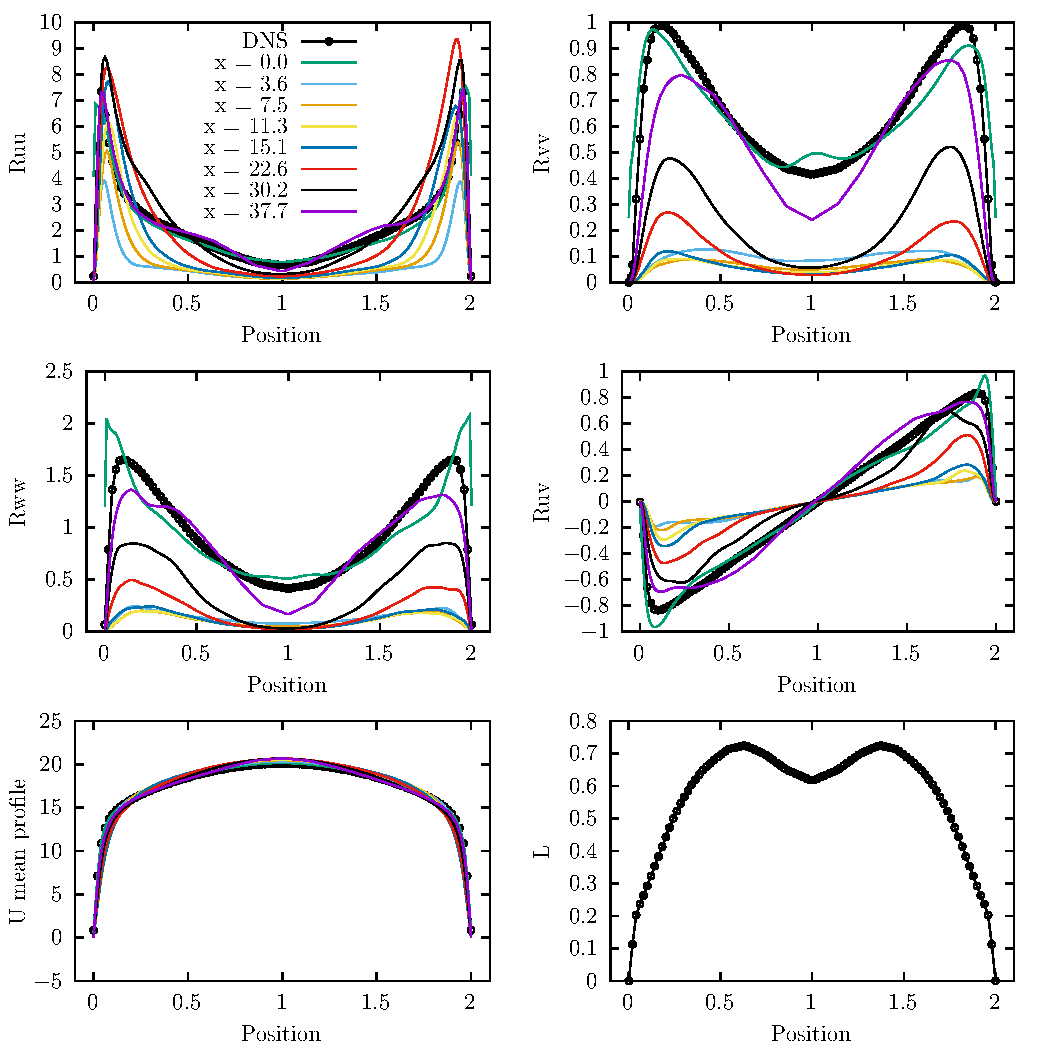
\includegraphics[width=0.95\textwidth]{URL_x.pdf}
  \caption{Time-averaged $U$, $\bR$ and $L$ along streamwise lines at
  various positions $x$, compared against the DNS target.}
  \label{fig:URL_x}
\end{figure*}

%%==============================================================================
\section{Usage}\label{sec:usage}
%%==============================================================================

\subsection{Setup}\label{sec:setup}

Once the source repository has been obtained:
\begin{enumerate}[noitemsep]
  \item Source your local OpenFOAM-12 environment as usual
    (e.g.\ \texttt{source etc/bashrc} in your OpenFOAM tree).
  \item Compile the boundary condition with \texttt{wmake} from the
    project root.
  \item Load the resulting library in your case's
    \texttt{system/controlDict}:
\begin{quote}\ttfamily\small
libs ("libsyntheticTurbulenceInlet.so");
\end{quote}
\end{enumerate}
Ready-to-run cases for each \texttt{geometryMode} are supplied under
\texttt{tutorials/}.
\Cref{tab:params} lists the dictionary entries accepted by the boundary
condition. 

\begin{table*}[ht]
\centering
\small
\begin{tabular}{@{}lll p{0.42\textwidth}@{}}
\toprule
Key & Type & Default & Description \\
\midrule
\multicolumn{4}{@{}l}{\itshape Mandatory}\\
\texttt{geometryMode} & word & --- &
  One of \texttt{annulus}, \texttt{disk}, \texttt{rectangle},
  \texttt{channel}, \texttt{arbitrary}.\\
\texttt{Umean} \emph{or} \texttt{massFlow} &
  \texttt{Function1<scalar>} & --- &
  Inlet target. \texttt{Umean} is read if \texttt{massFlowMode=false},
  \texttt{massFlow} otherwise.\\
\midrule
\multicolumn{4}{@{}l}{\itshape Optional}\\
\texttt{massFlowMode} & bool & \texttt{false} &
  \texttt{true}: read \texttt{massFlow} (kg/s).
  \texttt{false}: read \texttt{Umean} (m/s).\\
\texttt{wallLongOrShort} & word & \texttt{long} &
  Channel only: which side of the rectangle carries walls; the other is
  treated as periodic.\\
\texttt{arbitraryModeRadius} & scalar & max patch radius &
  Arbitrary mode only: radius within which to seed eddies.\\
\texttt{arbitraryModeCenter} & vector & patch centre &
  Arbitrary mode only: centre point for eddy seeding.\\
\texttt{Utau} & scalar & auto from \cref{eq:Colebrook} &
  Friction velocity. A negative value forces the lower limit
  $U_{\tau,\min}$, which maps the entire DNS profile across the
  available wall-to-wall distance.\\
\texttt{swirlNr} & scalar & \texttt{0} &
  Swirl number $S$. Annulus and disk only.\\
\texttt{d} & scalar & \texttt{1} &
  Eddy fill fraction $\sum V_k/V_0$.\\
\texttt{scale} & scalar & \texttt{1} (\texttt{0.2} for \texttt{arbitrary}) &
  Heuristic prefactor $s$ on $C_2$ (\Cref{eq:C2}).\\
\texttt{nCellPerEddy} & label & \texttt{1} (\texttt{5} for \texttt{arbitrary}) &
  Minimum eddy length in cell counts.\\
\texttt{Lref} & scalar & \texttt{1} &
  Length-scale normalisation for $L$.\\
\texttt{seed} & uint & \texttt{536} &
  Mersenne-Twister seed.\\
\texttt{rhoInf} & scalar & \texttt{1} &
  Reference density used by the incompressible mass-flow rescaling
  in~\Cref{eq:fCorr}.\\
\bottomrule
\end{tabular}
\caption{Dictionary entries accepted by \texttt{syntheticTurbulenceInlet}.}
\label{tab:params}
\end{table*}

A minimal patch entry is 

\noindent\begin{minipage}{\columnwidth}
\ttfamily\small
inlet\\
\{\\
\hspace*{2em}type\hspace{1.6em}syntheticTurbulenceInlet;\\
\hspace*{2em}geometryMode\hspace{0.3em}annulus;\\
\hspace*{2em}massFlowMode\hspace{0.3em}true;\\
\hspace*{2em}massFlow\hspace{1.0em}2.53e-4;\\
\}
\end{minipage}

%%==============================================================================
\noindent\begin{minipage}{\columnwidth}
\begin{thebibliography}{9}
\bibitem{PCR2013}
  Poletto, R., Craft, T., \& Revell, A.,
  \emph{A new divergence-free synthetic eddy method for the reproduction of
  inlet flow conditions for LES},
  Flow, Turbulence and Combustion, 91(3), 519--539, 2013.
  DOI:~\href{https://doi.org/10.1007/s10494-013-9488-2}{10.1007/s10494-013-9488-2}.

\bibitem{Fyhn2026Ammonia}
  Fyhn, H., Gruber, A., Nyg\aa rd, H.~T., Dawson, J., \& Nogenmyr, K.-J.,
  \emph{Numerical and Experimental Investigation of a Non-Premixed Flame
  of Partially Decomposed Ammonia at Atmospheric Pressure},
  Journal of Engineering for Gas Turbines and Power (submitted, 2026).

\bibitem{Fyhn2026FlameSheet}
  Fyhn, H., Meyer, O.~H.~H., Wang, Q., Worth, N., Koomen, J., Dammers, T., \& Gruber, A.,
  \emph{Numerical and Experimental Investigation of a Laboratory-Scale
  Hydrogen-Fired FlameSheet$^\text{TM}$ Burner Operated at Atmospheric
  Pressure With Full Optical Access},
  Journal of Engineering for Gas Turbines and Power (submitted, 2026).

\end{thebibliography}
\end{minipage}

\end{document}
